%% Creator: Inkscape inkscape 0.48.4, www.inkscape.org
%% PDF/EPS/PS + LaTeX output extension by Johan Engelen, 2010
%% Accompanies image file 'baysianmodel_limitedsensingcapability1.pdf' (pdf, eps, ps)
%%
%% To include the image in your LaTeX document, write
%%   \input{<filename>.pdf_tex}
%%  instead of
%%   \includegraphics{<filename>.pdf}
%% To scale the image, write
%%   \def\svgwidth{<desired width>}
%%   \input{<filename>.pdf_tex}
%%  instead of
%%   \includegraphics[width=<desired width>]{<filename>.pdf}
%%
%% Images with a different path to the parent latex file can
%% be accessed with the `import' package (which may need to be
%% installed) using
%%   \usepackage{import}
%% in the preamble, and then including the image with
%%   \import{<path to file>}{<filename>.pdf_tex}
%% Alternatively, one can specify
%%   \graphicspath{{<path to file>/}}
%% 
%% For more information, please see info/svg-inkscape on CTAN:
%%   http://tug.ctan.org/tex-archive/info/svg-inkscape
%%
\begingroup%
  \makeatletter%
  \providecommand\color[2][]{%
    \errmessage{(Inkscape) Color is used for the text in Inkscape, but the package 'color.sty' is not loaded}%
    \renewcommand\color[2][]{}%
  }%
  \providecommand\transparent[1]{%
    \errmessage{(Inkscape) Transparency is used (non-zero) for the text in Inkscape, but the package 'transparent.sty' is not loaded}%
    \renewcommand\transparent[1]{}%
  }%
  \providecommand\rotatebox[2]{#2}%
  \ifx\svgwidth\undefined%
    \setlength{\unitlength}{690.0328916bp}%
    \ifx\svgscale\undefined%
      \relax%
    \else%
      \setlength{\unitlength}{\unitlength * \real{\svgscale}}%
    \fi%
  \else%
    \setlength{\unitlength}{\svgwidth}%
  \fi%
  \global\let\svgwidth\undefined%
  \global\let\svgscale\undefined%
  \makeatother%
  \begin{picture}(1,0.27310058)%
    \put(0,0){\includegraphics[width=\unitlength]{baysianmodel_limitedsensingcapability1.pdf}}%
    \put(0.13491803,0.13096491){\color[rgb]{0,0,0}\makebox(0,0)[lb]{\smash{$F_0$}}}%
    \put(0.49896533,0.13042954){\color[rgb]{0,0,0}\makebox(0,0)[lb]{\smash{$F_{t-1}$}}}%
    \put(0.74302299,0.13011602){\color[rgb]{0,0,0}\makebox(0,0)[lb]{\smash{$F_t$}}}%
    \put(0.97065254,0.13132882){\color[rgb]{0,0,0}\makebox(0,0)[lb]{\smash{$C$}}}%
    \put(0.8592112,0.01748766){\color[rgb]{0,0,0}\makebox(0,0)[lb]{\smash{$S$}}}%
    \put(0.25259719,0.24338149){\color[rgb]{0,0,0}\makebox(0,0)[lb]{\smash{$U_0$}}}%
    \put(0.01344584,0.13000442){\color[rgb]{0,0,0}\makebox(0,0)[lb]{\smash{$Z_0$}}}%
    \put(0.13200121,0.01660858){\color[rgb]{0,0,0}\makebox(0,0)[lb]{\smash{$X_0$}}}%
    \put(0.25081942,0.1323528){\color[rgb]{0,0,0}\makebox(0,0)[lb]{\smash{$Z_1$}}}%
    \put(0.49567499,0.01710239){\color[rgb]{0,0,0}\makebox(0,0)[lb]{\smash{$X_{t-1}$}}}%
    \put(0.61582614,0.24265115){\color[rgb]{0,0,0}\makebox(0,0)[lb]{\smash{$U_{t-1}$}}}%
    \put(0.62760963,0.13166754){\color[rgb]{0,0,0}\makebox(0,0)[lb]{\smash{$Z_t$}}}%
    \put(0.74474442,0.01791113){\color[rgb]{0,0,0}\makebox(0,0)[lb]{\smash{$X_t$}}}%
    \put(0.97294884,0.24531693){\color[rgb]{0,0,0}\makebox(0,0)[lb]{\smash{$T$}}}%
    \put(0.85629863,0.24349111){\color[rgb]{0,0,0}\makebox(0,0)[lb]{\smash{$U_t$}}}%
    \put(0.36449826,0.01670913){\color[rgb]{0,0,0}\makebox(0,0)[lb]{\smash{$X_1$}}}%
    \put(0.36582879,0.13197239){\color[rgb]{0,0,0}\makebox(0,0)[lb]{\smash{$F_1$}}}%
    \put(0.48245853,0.24385444){\color[rgb]{0,0,0}\makebox(0,0)[lb]{\smash{$U_1$}}}%
  \end{picture}%
\endgroup%
